\documentclass[12pt,letterpaper]{article}
\usepackage{pdfpages}
\usepackage{fancyhdr}
\usepackage{tablefootnote}
\usepackage{array}
\usepackage{colortbl}
\usepackage[colorlinks=true, urlcolor=blue, linkcolor=blue]{hyperref}
\usepackage{graphicx}
\usepackage[top=1.4in, left=0.5in, right=0.5in, bottom=0.8in]{geometry}
\usepackage[T1]{fontenc}
\usepackage{helvet}
\usepackage{booktabs}
\usepackage[table,xcdraw]{xcolor}
\pagestyle{fancy}
\renewcommand{\headrulewidth}{0pt}
\renewcommand{\footrulewidth}{0pt}
\setlength{\parindent}{0em}
\setlength{\parskip}{1em}


\fancyfoot[C]{\setlength{\unitlength}{1in}\begin{picture}(5,0)\put(-1.8,-1){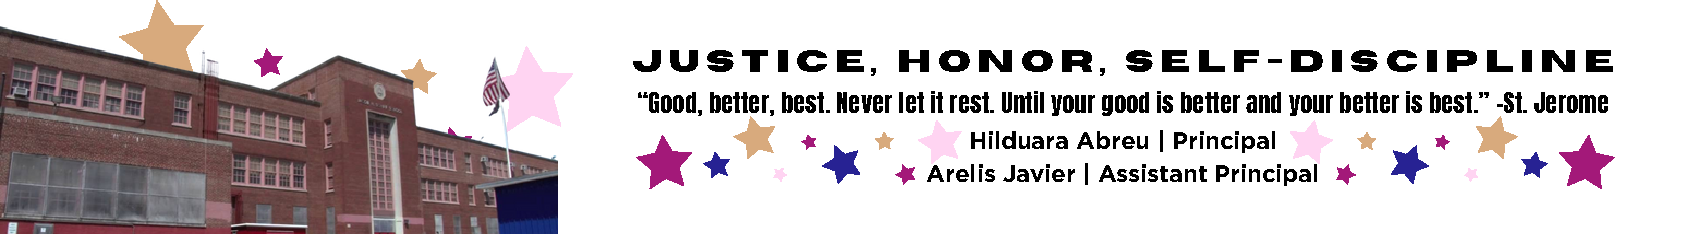
\includegraphics[width=8.8in,height=1.3in]{logo-1}}\end{picture}}
\fancyhead[C]{\setlength{\unitlength}{1in}\begin{picture}(5,0)\put(-1.9,-1){
\includegraphics[width=8.9in,height=1.3in]{logo-2}}\end{picture}}

\pagenumbering{gobble}
\addtolength{\evensidemargin}{-2in}
\addtolength{\topmargin}{-0.5in}
\addtolength{\textwidth}{0in}
%%%%%%%%%%%%%%%%%%%%%%%%%%%%%%%%%%%%%%%%%%%%%%%%%%%%%%%%%%%%%%%%%%

\begin{document}
\vspace*{0.5in}
School Year: \href{https://www.ps192.org}{2024-25} 

\textbf{Sujeto: Horario Escolar}

Un horario escolar especifica la hora de inicio y la duración de uno o más períodos de instrucción de cada día. Un horario diario consistente y rutinario
les ofrece a los niños una disciplina de trabajo durante la semana de clase. Un
horario escolar ayuda a los niños a:
\begin{itemize}
\item Sentirse en control de su entorno.
\item Sentirse seguro, protegido y cómodo.
\item Poder realizar una actividad o tarea.
\item Participar en el aprendizaje.
\end{itemize}
Al igual que los adultos, los niños se sienten más confiados y seguros cuando sus
actividades diarias son predecibles y familiares.

\begin{table}[h]
\centering
\begin{tabular}{|>{\centering\hspace{0pt}}m{0.146\linewidth}|>{\centering\hspace{0pt}}m{0.23\linewidth}|>{\centering\hspace{0pt}}m{0.213\linewidth}|>{\centering\arraybackslash\hspace{0pt}}m{0.315\linewidth}|} 
\hline
\rowcolor[rgb]{1,0.745,0.435} Periodo & Comienzo & Termino & Duracion                                                                      \\ 
\hline
1                                    & 08:00 AM   & 08:45 AM & 45 minutes                                                                  \\ 
\hline
\rowcolor[rgb]{0.6,0.757,0.945} 2    & 08:45 AM   & 09:30 AM & 45 minutes                                                                  \\ 
\hline
3                                    & 09:30 AM   & 10:15 AM & 45 minutes                                                                  \\ 
\hline
\rowcolor[rgb]{0.6,0.757,0.945} 4    & 10:15 AM   & 11:05 AM & 50 minutes                                                                  \\ 
\hline
5                                    & 11:05 AM   & 11:55 AM & 50 minutes  \\ 
\hline
\rowcolor[rgb]{0.6,0.757,0.945} 6    & 11:55 AM   & 12:40 PM & 45 minutes \\ 
\hline
7                                    & 12:40 PM   & 01:30 PM & 50 minutes                                                                  \\ 
\hline
\rowcolor[rgb]{0.6,0.757,0.945} 8    & 01:30 PM   & 02:15 PM & 45 minutes                                                                  \\
\hline
\end{tabular}
\end{table}

En Union,


\includegraphics[width=0.2\textwidth]{hil_signature}

\textbf{Principal}

\textit{La Escuela donde El Aprendisaje es Divertido!}

\url{www.ps192.org}


\end{document}
